\documentclass[conference,compsoc]{IEEEtran}
\usepackage[utf8]{inputenc}
\usepackage[T1]{fontenc}
\usepackage{amsmath,amssymb,amsthm}
\usepackage{booktabs}
\usepackage{graphicx}
\usepackage{xcolor}
\usepackage{hyperref}
\usepackage{array}

\newtheorem{theorem}{Theorem}
\newtheorem{definition}{Definition}

\title{Stateless Post-Quantum Threshold Custody and Knowledge-Asymmetry Frozen UTXO Rescue:\\
Resolving Multi-Zone State Hazards and Legacy Quantum Sunset Risks}

\author{
  \IEEEauthorblockN{Laudza Kusuma}
  \IEEEauthorblockA{Independent Researcher, Depok, Indonesia\\
  Email: laudzaxie@gmail.com\\
  Web: \url{https://laudzakusuma.github.io}}
}

\begin{document}
\maketitle

\begin{abstract}
Publishing AQMP v2.0 (Zenodo Record 24303569) established formal byte-footprint equations, deterministic aggregation thresholds, and QROM soundness for standard transactions. Two critical open problems remained in late-2026 post-quantum cryptocurrency engineering. First, institutional custodians replicate signing shares across isolated availability zones and restore nodes from cold backups, making stateful post-quantum signatures unusable whenever counter reuse leaks signing keys. Second, roughly 34\% of Bitcoin supply rests in legacy outputs vulnerable to quantum key recovery or scheduled sunsetting under draft BIP-361, yet existing rescue schemes expose raw public keys or ship multi-kilobyte witnesses.

This paper resolves both bottlenecks with two interoperable constructions. First, we build a \textbf{Stateless Post-Quantum Threshold Signature Engine} over $\mathbb{F}_q^{64}$ ($q = 8{,}380{,}417$) using Shamir polynomial sharing and synthetic PRF nonce derivation bound to message digest, share commitment, active signer set $S$, and an immutable epoch salt. Because signers hold zero mutable signing counters, wiping local memory and restoring from cold backup yields identical partial signatures on repeated inputs and independent nonces across distinct messages. Bound to BIP-360 P2MR roots and AQMP v2.0 4-byte \texttt{KeyRegistry} indexing, a $3$-of-$5$ custody quorum executes signing in $36.48\text{ ms}$ ($3.97\text{ ms}$ group verification) while shrinking $250$-transaction block payloads to $11{,}300\text{ B}$ ($-99.71\%$ relative to $3$-of-$5$ ML-DSA-65). Second, we construct a \textbf{Knowledge-Asymmetry Frozen UTXO Rescue Protocol} that proves knowledge of an unhardened BIP-32 parent chain code $c_{\text{par}}$ via a post-quantum module-lattice proof of knowledge over $\mathbb{F}_q^{32}$ without exposing $P_{\text{par}}$ or $P_{\text{child}}$ in plaintext. The compact rescue witness occupies exactly $580\text{ B}$ ($32\text{ B}$ chain-code commitment, $64\text{ B}$ lattice PoK transcript, $164\text{ B}$ Merkle snapshot proof, and $320\text{ B}$ destination NIZK) paired with a $96\text{ B}$ Dual-Commit XOR cycle ($676\text{ B}$ total, $-87.2\%$ relative to Naive ML-DSA-65) gated by Fukuda's window $\Delta_{\text{eff}} \ge \lceil 4/(1-\epsilon)\rceil$.
\end{abstract}

\section{Introduction}
\label{sec:intro}

Post-quantum migration designs for Bitcoin and Ethereum must handle operational failure modes beyond single-key EOA transfers. Institutional custody clusters deploy $t$-of-$n$ signing thresholds across geographically separated availability zones where virtual-machine snapshots, failover promotions, and cold-backup restores routinely reset volatile RAM and disk state. Stateful hash-based signature schemes (XMSS, LMS) suffer catastrophic secret-key recovery if any backup restoration repeats a one-time signature index. Lattice threshold designs built on random ephemeral nonces face the same hazard when crash recovery replays an intermediate signing round with fresh randomness over an already-used polynomial commitment.

At the protocol layer, approximately 34\% of circulating Bitcoin sits in legacy P2PK, reused P2PKH, P2WPKH, and exposed Taproot outputs susceptible to Shor's algorithm on a Cryptographically Relevant Quantum Computer (CRQC). Draft proposals such as BIP-360 (P2MR) and BIP-361 address new or voluntarily migrated coins, while emergency sweep designs (Lifeboat, Dropkick) demand $3{,}420\text{ B}$ to $5{,}261\text{ B}$ on-chain per rescued coin or risk mempool destination hijacking if an adversary recovers the classical ECDSA key during broadcast.

Building on AQMP v2.0 (Zenodo Record 24303569), we present and benchmark two reference modules:
\begin{enumerate}
    \item \textbf{Stateless PQ-MPC Threshold Signing (\texttt{stateless\_pq\_mpc.py}):} Eliminates mutable signing counters through deterministic synthetic HMAC-SHA3-256 nonces, constant-time vector verification, and native BIP-360 P2MR plus 4-byte \texttt{KeyRegistry} compatibility.
    \item \textbf{Knowledge-Asymmetry Frozen UTXO Rescue (\texttt{utxo\_rescue.py}):} Replaces plaintext elliptic-curve exposure with a $580\text{ B}$ post-quantum lattice PoK of an unhardened BIP-32 chain code $c_{\text{par}}$ bound to a $96\text{ B}$ Dual-Commit XOR cycle and Fukuda confirmation deadline $\Delta^* = \lceil 4/(1-\epsilon)\rceil$.
\end{enumerate}

\section{Stateless Post-Quantum Threshold Custody}
\label{sec:mpc}

\subsection{Key Sharing and Synthetic PRF Nonces}
Let $q = 8{,}380{,}417$ and $d = 64$. A setup dealer (or distributed key generation ceremony) samples a master secret $\mathbf{s} \in \mathbb{F}_q^d$ and public matrix $\mathbf{A} \in \mathbb{F}_q^{d \times d}$ from a 32-byte seed, publishing $\mathbf{b} = \mathbf{A}\mathbf{s} \bmod q$. For each coordinate $k \in \{0, \dots, d-1\}$, a degree-$(t-1)$ Shamir polynomial evaluates $s_{i,k} = f_k(i) \bmod q$ for signer $i \in \{1, \dots, n\}$. Signer $i$ stores an immutable cold-backup tuple:
\begin{equation}
\mathsf{Share}_i = \big(i, t, n, \mathbf{s}_i, k_i, \mathsf{com}_i, \mathsf{seed}_{\mathbf{A}}, \mathbf{b}\big),
\end{equation}
where $\mathsf{com}_i = \mathbf{A}\mathbf{s}_i \bmod q$ and $k_i \xleftarrow{\$} \{0,1\}^{256}$ is a static PRF root key. By design, $\mathsf{Share}_i$ contains no mutable counter or monotonic state register.

To sign message $m$ under active signer quorum $S \subseteq \{1,\dots,n\}$ ($|S|=t$) and backup-safe epoch salt $\sigma$, signer $i$ derives its synthetic nonce deterministically:
\begin{equation}
r_i = \mathrm{HMAC\text{-}SHA3\text{-}256}\Big(k_i,\; \texttt{"AQMP\_STATELESS\_NONCE\_v2:"} \parallel H(m) \parallel H(\mathsf{com}_i) \parallel \mathrm{enc}(S) \parallel \sigma\Big).
\end{equation}
Expanding $r_i$ via SHA3-512 yields $\mathbf{y}_i \in \mathbb{F}_q^d$ and nonce commitment $\mathbf{w}_i = \mathbf{A}\mathbf{y}_i \bmod q$. With $\mathbf{W} = \sum_{i \in S} \mathbf{w}_i \bmod q$ and Fiat-Shamir challenge
\begin{equation}
c = H_{\mathbb{F}_q}\big(\mathsf{seed}_{\mathbf{A}} \parallel \mathbf{b} \parallel \mathbf{W} \parallel H(m) \parallel \mathsf{root}_{\text{P2MR}} \parallel \mathsf{idx}_{\text{KeyReg}}\big),
\end{equation}
signer $i$ computes partial signature $\mathbf{z}_i = \mathbf{y}_i + c \cdot \lambda_{i,S} \cdot \mathbf{s}_i \bmod q$, where $\lambda_{i,S} = \prod_{j \in S, j \ne i} \frac{-j}{i-j} \bmod q$.

\subsection{Constant-Time Verification and Backup-Restore Safety}
Every partial share satisfies $\mathbf{A}\mathbf{z}_i \equiv \mathbf{w}_i + (c\lambda_{i,S})\mathsf{com}_i \pmod q$, and the combined threshold signature $(\mathbf{W}, \mathbf{z} = \sum_{i \in S}\mathbf{z}_i \bmod q)$ satisfies:
\begin{equation}
\mathbf{A}\mathbf{z} - c\mathbf{b} = \mathbf{A}\left(\sum_{i \in S}\mathbf{y}_i + c\sum_{i \in S}\lambda_{i,S}\mathbf{s}_i\right) - c(\mathbf{A}\mathbf{s}) \equiv \mathbf{W} \pmod q.
\end{equation}
All vector operations execute in fixed-length loops over $d = 64$ coordinates and finalize equality via constant-time \texttt{hmac.compare\_digest}. Wiping volatile node state and restoring $\mathsf{Share}_i$ from cold backup reproduces identical $(\mathbf{w}_i, \mathbf{z}_i)$ for identical $(m, S, \sigma)$ and fresh pseudorandom nonces for any new message $m' \ne m$, eliminating backup-replay key leakage.

\subsection{BIP-360 P2MR and AQMP v2.0 KeyRegistry Integration}
Binding the 32-byte BIP-360 P2MR Merkle root and 4-byte \texttt{KeyRegistry} index directly into $c$ enables $t$-of-$n$ signatures to fold into Plonky3 BabyBear recursive proofs at $300 + 44N\text{ B}$ per block. For $N = 250$ transactions under $3$-of-$5$ custody, block payload shrinks from $3{,}945{,}750\text{ B}$ (naive $3$-of-$5$ ML-DSA-65) and $517{,}500\text{ B}$ ($3$-of-$5$ P2MR FALCON-KR) down to $11{,}300\text{ B}$ ($-99.71\%$).

\section{Knowledge-Asymmetry Frozen UTXO Rescue}
\label{sec:rescue}

\subsection{Why Unhardened BIP-32 Chain Codes Create Quantum Asymmetry}
In an unhardened BIP-32 wallet, child public key $P_{\text{child}} = P_{\text{par}} + I_L \cdot G$ depends on $(I_L \parallel I_R) = \mathrm{HMAC\text{-}SHA512}(c_{\text{par}}, P_{\text{par}} \parallel i)$, while the legacy Bitcoin script commits only to $\mathrm{Hash160}(P_{\text{child}})$. Even a CRQC that recovers $sk_{\text{child}}$ from an exposed $P_{\text{child}}$ cannot invert HMAC-SHA512 to learn the 256-bit parent chain code $c_{\text{par}}$. Only the legitimate owner holds $c_{\text{par}}$ together with $(P_{\text{par}}, i)$.

\subsection{580-Byte Rescue Witness and Dual-Commit XOR Binding}
To avoid publishing $P_{\text{par}}$, $P_{\text{child}}$, or $c_{\text{par}}$ in plaintext on-chain, the owner derives a private post-quantum lattice key $\mathbf{s}_{\text{KA}} \in \mathbb{F}_q^{32}$ from $\mathrm{HMAC\text{-}SHA3\text{-}256}(c_{\text{par}}, P_{\text{par}} \parallel i \parallel \mathrm{addr})$ and anchors its pre-sunset tag $H(\mathbf{b}_{\text{KA}} \parallel \mathsf{utxo\_id} \parallel \mathrm{addr})$ where $\mathbf{b}_{\text{KA}} = \mathbf{A}_{\text{KA}}\mathbf{s}_{\text{KA}} \bmod q$. Rescue claims serialize a fixed $580\text{ B}$ witness:
\begin{equation}
|\mathsf{Witness}_{\text{rescue}}| = \underbrace{32\text{ B}}_{\kappa \text{ commit}} + \underbrace{64\text{ B}}_{(h_w, c_{\text{FS}})} + \underbrace{164\text{ B}}_{\text{Merkle proof}} + \underbrace{320\text{ B}}_{(\mathbf{z}_{\text{KA}}, \mathbf{b}_{\text{KA}}, \mathsf{tag}_{\text{dest}})} = 580\text{ B}.
\end{equation}
On-chain validators verify snapshot Merkle inclusion against $\mathsf{root}_{\text{UTXO}}$, confirm $\mathbf{b}_{\text{KA}}$ matches the frozen UTXO tag, check the Fiat-Shamir challenge $c_{\text{FS}}$, and verify $\mathbf{A}_{\text{KA}}\mathbf{z}_{\text{KA}} - c\mathbf{b}_{\text{KA}} \equiv \mathbf{w}_{\text{KA}} \pmod q$.

To block mempool destination hijacking during rescue, the $580\text{ B}$ witness binds into a $96\text{ B}$ AQMP v2.0 Dual-Commit XOR cycle:
\begin{equation}
\text{Commit Tx1 (32 B): } C = F(x) \oplus F(x \parallel m_{\text{rescue}}), \qquad \text{Reveal Tx2 (64 B): } (x, y' = F(x')),
\end{equation}
where $m_{\text{rescue}}$ encodes $(\mathsf{utxo\_id}, \mathsf{satoshis}, \mathsf{pqc\_dest}, \kappa, h_w, c_{\text{FS}})$. Consensus enforces Fukuda's confirmation window $\Delta_{\text{eff}} \ge \Delta^*(\epsilon) = \lceil 4/(1-\epsilon)\rceil$ before Tx2 finalizes. Total on-chain rescue payload is $580 + 96 = 676\text{ B}$.

\section{Formal Security Model and Proofs}
\label{sec:security}

We formalize unforgeability for both constructions in self-contained reduction proofs suitable for independent verification.

\begin{definition}[TS-UF-CMA with Cold-Backup Resets]
Let $\Pi_{\mathrm{MPC}}$ be a $t$-of-$n$ stateless threshold signature scheme over $\mathbb{F}_q^d$. In experiment $\mathsf{Exp}^{\mathrm{TS\text{-}UF\text{-}CMA}}_{\Pi_{\mathrm{MPC}}}(\mathcal{A})$, adversary $\mathcal{A}$ corrupts a subset $\mathcal{C} \subset \{1, \dots, n\}$ of size $|\mathcal{C}| \le t - 1$, receives $\{\mathsf{Share}_j\}_{j \in \mathcal{C}}$ together with public key $(\mathsf{seed}_{\mathbf{A}}, \mathbf{b}, \{\mathsf{com}_i\}_{i=1}^n)$, and makes up to $q_H$ random oracle queries and $q_S$ partial signing queries on tuples $(i, m, S, \sigma)$ for honest signers $i \notin \mathcal{C}$. At any point, $\mathcal{A}$ may issue a $\mathsf{Reset}(i)$ oracle call wiping volatile memory on node $i$ and restoring $\mathsf{Share}_i$ from cold backup. $\mathcal{A}$ wins if it outputs $(m^*, \mathbf{W}^*, \mathbf{z}^*, c^*)$ verifying under $\mathbf{b}$ such that $m^*$ was never queried to a full signing quorum of size $t$.
\end{definition}

\begin{definition}[Rescue-QROM Soundness and Anti-Front-Running]
In experiment $\mathsf{Exp}^{\mathrm{Rescue\text{-}QROM}}(\mathcal{A})$, the challenger samples an unhardened BIP-32 wallet $(c_{\mathrm{par}}, P_{\mathrm{par}}, i)$ producing frozen output $\mathrm{Hash160}(P_{\mathrm{child}})$ and snapshot tag $H(\mathbf{b}_{\mathrm{KA}} \parallel \mathsf{utxo\_id} \parallel \mathrm{addr})$ inside $\mathsf{root}_{\mathrm{UTXO}}$. Adversary $\mathcal{A}$ is given $P_{\mathrm{child}}$, the classical ECDSA secret key $sk_{\mathrm{child}}$ (modeling a full CRQC break of secp256k1), and the public Commit Tx1 $C = F_{\mathrm{PRE}}(x) \oplus F_{\mathrm{MSG}}(x \parallel m_{\mathrm{rescue}})$ while making at most $q_F$ quantum superposition queries to $F$ prior to Reveal Tx2 within Fukuda's window $\Delta_{\text{eff}} \ge \Delta^*(\epsilon)$. $\mathcal{A}$ wins if it outputs a valid $676\text{ B}$ rescue bundle redirecting the frozen UTXO to an adversarial destination $\mathsf{pqc\_dest}^* \ne \mathsf{pqc\_dest}$.
\end{definition}

\begin{theorem}[Stateless PQ-MPC Unforgeability and Backup-Reset Safety]
\label{thm:mpc}
Assuming $\mathrm{HMAC\text{-}SHA3\text{-}256}$ is a secure PRF and the underlying module-lattice relation $\mathbf{A}\mathbf{s} \equiv \mathbf{b} \pmod q$ is hard against key recovery, for any adversary $\mathcal{A}$ corrupting at most $t - 1$ signers and making $q_H$ random oracle queries and $q_S$ signing queries (including arbitrary cold-backup resets),
\begin{equation}
\mathrm{Adv}^{\mathrm{TS\text{-}UF\text{-}CMA}}_{\Pi_{\mathrm{MPC}}}(\mathcal{A})
\le (n - t + 1)\,\mathrm{Adv}^{\mathrm{PRF}}_{\mathrm{HMAC}}(\mathcal{B}_{\mathrm{PRF}}) + \sqrt{q_H \cdot \mathrm{Adv}^{\mathrm{MLWE/MSIS}}_{\mathbb{F}_q^d}(\mathcal{B}_{\mathrm{Lat}})} + \frac{q_H + q_S}{q}.
\end{equation}
\end{theorem}

\begin{proof}
We transition through three games $G_0 \to G_1 \to G_2$:

\textbf{Game 0 (Real Execution):} $\mathcal{A}$ interacts with the real $\mathsf{Exp}^{\mathrm{TS\text{-}UF\text{-}CMA}}_{\Pi_{\mathrm{MPC}}}(\mathcal{A})$ challenger. Because $\mathsf{Share}_i$ contains no mutable state register, every $\mathsf{Reset}(i)$ call leaves $\mathsf{Share}_i$ bit-identical, so $\mathrm{Adv}^{\mathrm{TS\text{-}UF\text{-}CMA}}_{\Pi_{\mathrm{MPC}}}(\mathcal{A}) = \Pr[G_0]$.

\textbf{Game 1 (PRF-to-Random Nonce Table Replacement):} For each honest signer $i \notin \mathcal{C}$, replace $r_i = \mathrm{HMAC\text{-}SHA3\text{-}256}(k_i, \cdot)$ with an internal lazy random function table $T_i[m, \mathsf{com}_i, S, \sigma]$. Repeated queries after $\mathsf{Reset}(i)$ on the same $(m, S, \sigma)$ return the identical cached nonce $\mathbf{y}_i$ (preserving exact backup-restore determinism), while every fresh tuple $(m', S', \sigma')$ receives an independent uniform nonce $\mathbf{y}_i' \xleftarrow{\$} \mathbb{F}_q^d$. By a standard hybrid argument over the $n - |\mathcal{C}| \le n - t + 1$ honest signers,
\begin{equation}
|\Pr[G_0] - \Pr[G_1]| \le (n - t + 1)\,\mathrm{Adv}^{\mathrm{PRF}}_{\mathrm{HMAC}}(\mathcal{B}_{\mathrm{PRF}}).
\end{equation}

\textbf{Game 2 (Zero-Knowledge Simulation and General Forking Lemma):} Given a lattice challenge instance $(\mathbf{A}, \mathbf{b})$, the reduction $\mathcal{B}_{\mathrm{Lat}}$ samples the $|\mathcal{C}| \le t - 1$ corrupted shares $\{\mathbf{s}_j\}_{j \in \mathcal{C}}$ uniformly from $\mathbb{F}_q^d$, which fixes the public commitments $\mathsf{com}_i$ of all honest signers $i \notin \mathcal{C}$ via Lagrange interpolation in the linear exponent using $\mathbf{b}$. On each honest partial signing query, $\mathcal{B}_{\mathrm{Lat}}$ samples $\mathbf{z}_i \xleftarrow{\$} \mathbb{F}_q^d$, programs the Fiat-Shamir challenge $c \xleftarrow{\$} \mathbb{F}_q$ on $(\mathbf{W}, H(m), \mathsf{root}_{\text{P2MR}}, \mathsf{idx}_{\text{KeyReg}})$, and sets $\mathbf{w}_i = \mathbf{A}\mathbf{z}_i - (c\lambda_{i,S})\mathsf{com}_i \bmod q$, aborting only on an accidental oracle collision (probability at most $(q_H + q_S)/q$). By the General Forking Lemma~\cite{bellare2006}, rewinding a successful forger $\mathcal{A}$ on the target query yields two valid forgeries $(\mathbf{W}^*, c_1, \mathbf{z}_1)$ and $(\mathbf{W}^*, c_2, \mathbf{z}_2)$ with $c_1 \ne c_2 \bmod q$ with probability at least $\Pr[G_2]^2 / q_H - 1/q$. Subtracting the two verification equations gives:
\begin{equation}
\mathbf{A}(\mathbf{z}_1 - \mathbf{z}_2) \equiv (c_1 - c_2)\mathbf{b} \pmod q,
\end{equation}
which extracts $\mathbf{s}^* = (c_1 - c_2)^{-1}(\mathbf{z}_1 - \mathbf{z}_2) \bmod q$ satisfying $\mathbf{A}\mathbf{s}^* \equiv \mathbf{b} \pmod q$, bounding $\Pr[G_2] \le \sqrt{q_H \cdot \mathrm{Adv}^{\mathrm{MLWE/MSIS}}_{\mathbb{F}_q^d}(\mathcal{B}_{\mathrm{Lat}})} + (q_H + q_S)/q$. Combining the game hops completes the proof.
\end{proof}

\begin{theorem}[676-Byte UTXO Rescue Soundness and QROM Front-Running Resistance]
\label{thm:rescue}
Let $F : \{0,1\}^* \to \{0,1\}^n$ be modeled as a quantum random oracle under Zhandry's compressed oracle framework~\cite{zhandry2019}. For any quantum adversary $\mathcal{A}$ making at most $q_F$ superposition queries before Reveal Tx2 (even when $\mathcal{A}$ holds the compromised classical key $sk_{\mathrm{child}}$),
\begin{equation}
\mathrm{Adv}^{\mathrm{Rescue\text{-}QROM}}(\mathcal{A})
\le \mathrm{Adv}^{\mathrm{PoK/MSIS}}_{\mathbb{F}_q^{32}}(\mathcal{B}_1)
+ \mathrm{Adv}^{\mathrm{Pre}}_{\mathrm{HMAC\text{-}SHA512}}(\mathcal{B}_2)
+ \frac{8(q_F + 1)^2 + 32 q_F^3}{2^n}
+ \mathrm{negl}(\lambda).
\end{equation}
\end{theorem}

\begin{proof}
An adversary winning $\mathsf{Exp}^{\mathrm{Rescue\text{-}QROM}}(\mathcal{A})$ must either (Case~A) forge the $580\text{ B}$ Knowledge-Asymmetry witness for an adversarial destination $\mathsf{pqc\_dest}^* \ne \mathsf{pqc\_dest}$ without possessing $c_{\mathrm{par}}$, or (Case~B) hijack an in-flight honest rescue by forging a Dual-Commit XOR reveal $(x^*, m^*_{\mathrm{rescue}})$ matching Commit Tx1 $C$ before honest Reveal Tx2 settles.

\textbf{Case A (Knowledge Extraction of $c_{\mathrm{par}}$):} To pass snapshot verification, $\mathbf{b}_{\mathrm{KA}}$ is fixed by the pre-sunset commitment $\mathrm{public\_asymmetry\_tag} = H(\mathbf{b}_{\mathrm{KA}} \parallel \mathsf{utxo\_id} \parallel \mathrm{addr})$ inside $\mathsf{root}_{\mathrm{UTXO}}$. Rewinding the Fiat-Shamir lattice PoK $(h_w, c_{\mathrm{FS}}, \mathbf{z}_{\mathrm{KA}})$ over $\mathbb{F}_q^{32}$ extracts a valid witness $\mathbf{s}_{\mathrm{KA}}$ satisfying $\mathbf{A}_{\mathrm{KA}}\mathbf{s}_{\mathrm{KA}} \equiv \mathbf{b}_{\mathrm{KA}} \pmod q$ (bounded by $\mathrm{Adv}^{\mathrm{PoK/MSIS}}_{\mathbb{F}_q^{32}}(\mathcal{B}_1)$). Because $\mathbf{s}_{\mathrm{KA}}$ is derived from $\mathrm{HMAC\text{-}SHA3\text{-}256}(c_{\mathrm{par}}, P_{\mathrm{par}} \parallel i \parallel \mathrm{addr})$ and $c_{\mathrm{par}}$ is a $256$-bit symmetric key never revealed by $P_{\mathrm{child}}$ or $sk_{\mathrm{child}}$, recovering $c_{\mathrm{par}}$ reduces to inverting HMAC-SHA512 ($\mathrm{Adv}^{\mathrm{Pre}}_{\mathrm{HMAC\text{-}SHA512}}(\mathcal{B}_2)$).

\textbf{Case B (Zhandry QROM Front-Running Bound):} Given honest Commit Tx1 $C = F_{\mathrm{PRE}}(x) \oplus F_{\mathrm{MSG}}(x \parallel m_{\mathrm{rescue}})$ locked for $\Delta_{\text{eff}} \ge \Delta^*(\epsilon)$ blocks before $x$ is revealed, substituting $\mathsf{pqc\_dest}^* \ne \mathsf{pqc\_dest}$ yields $m^*_{\mathrm{rescue}} \ne m_{\mathrm{rescue}}$. By Zhandry's compressed oracle purification and the O2H reprogramming lemma~\cite{zhandry2019,aqmp2026}, any quantum adversary making $q_F$ superposition queries to $F$ hits preimage $x$ with probability at most $8(q_F + 1)^2 / 2^n$ or finds an oracle collision with probability at most $32 q_F^3 / 2^n$. Taking a union bound over Cases~A and~B yields the stated bound.
\end{proof}

\section{Empirical Benchmarks and Security Verification}
\label{sec:benchmarks}

We benchmarked both modules in \texttt{research/benchmark\_paper2\_mpc\_rescue.py} and validated all invariants via 59 automated pytest checks (\texttt{test\_paper2\_mpc\_rescue.py} plus AQMP v2.0 and QROM suites). Table~\ref{tab:mpc} and Fig.~\ref{fig:mpc} report measured quorum latency and block payload scaling across $t$-of-$n$ custody committees. Table~\ref{tab:rescue} and Fig.~\ref{fig:rescue} compare our $676\text{ B}$ UTXO rescue cycle against Lifeboat ($3{,}420\text{ B}$), Dropkick ($3{,}904\text{ B}$), and Naive ML-DSA-65 ($5{,}261\text{ B}$), alongside measured proof creation ($1.97\text{ ms}$ mean) and verification ($1.05\text{ ms}$ mean) latency under Fukuda gating ($\Delta^* \in \{5, 6, 8, 16, 40\}$).

\begin{table}[t]
\centering
\caption{Stateless PQ-MPC Latency and Block Payload ($N = 250$ Tx/Block)}
\label{tab:mpc}
\begin{tabular}{@{}ccccc@{}}
\toprule
Quorum ($t$-of-$n$) & Sign (ms) & Verify (ms) & Plonky3 + KeyReg (B) & Naive $t$-ML-DSA-65 (B) \\
\midrule
2-of-3 & 24.38 & 4.68 & 11,300 & 2,630,500 \\
3-of-5 & 36.48 & 3.97 & 11,300 & 3,945,750 \\
4-of-7 & 50.82 & 4.40 & 11,300 & 5,261,000 \\
5-of-9 & 66.82 & 4.32 & 11,300 & 6,576,250 \\
7-of-11 & 87.73 & 3.90 & 11,300 & 9,206,750 \\
\bottomrule
\end{tabular}
\end{table}

\begin{table}[t]
\centering
\caption{Frozen UTXO Rescue Footprint Comparison}
\label{tab:rescue}
\begin{tabular}{@{}lrr@{}}
\toprule
Rescue Scheme & Total On-Chain Bytes & Reduction vs.\ ML-DSA-65 \\
\midrule
AQMP Knowledge-Asymmetry Rescue (580B + 96B DCL) & \textbf{676 B} & \textbf{87.15\%} \\
Lifeboat (Commit-Delay-Reveal + PQC) & 3,420 B & 34.99\% \\
Dropkick (ZK Seed Recovery Proof) & 3,904 B & 25.79\% \\
Naive ML-DSA-65 Spend (Baseline) & 5,261 B & 0.00\% \\
\bottomrule
\end{tabular}
\end{table}

\begin{figure*}[t]
\centering
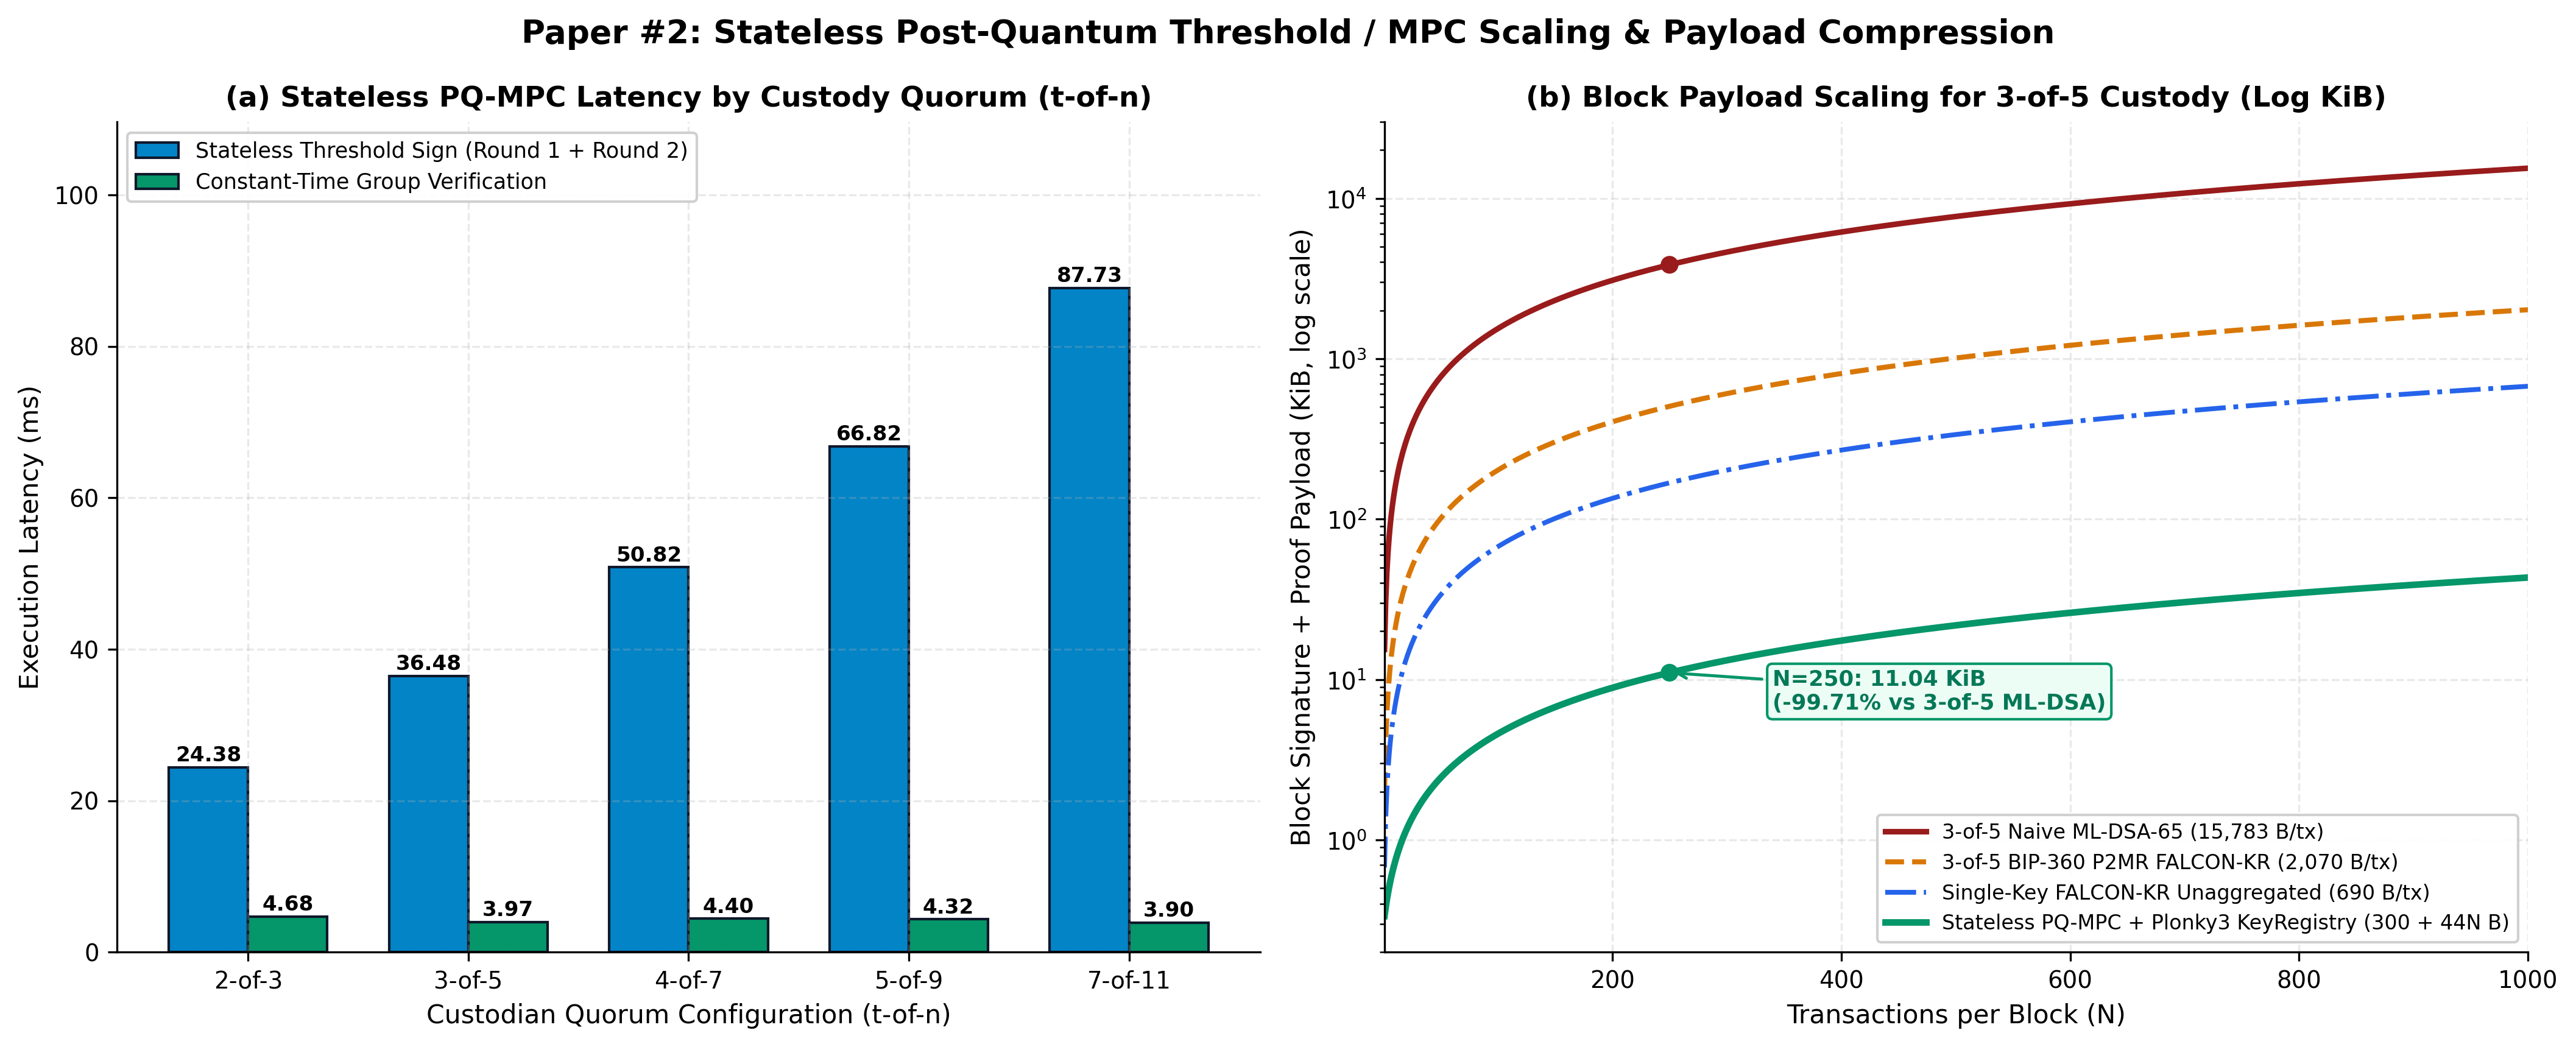
\includegraphics[width=0.95\textwidth]{figures/fig4_stateless_mpc_scaling.png}
\caption{Stateless PQ-MPC threshold execution latency across custody quorums (left) and block-level payload scaling under 3-of-5 custody with Plonky3 + KeyRegistry aggregation (right).}
\label{fig:mpc}
\end{figure*}

\begin{figure*}[t]
\centering
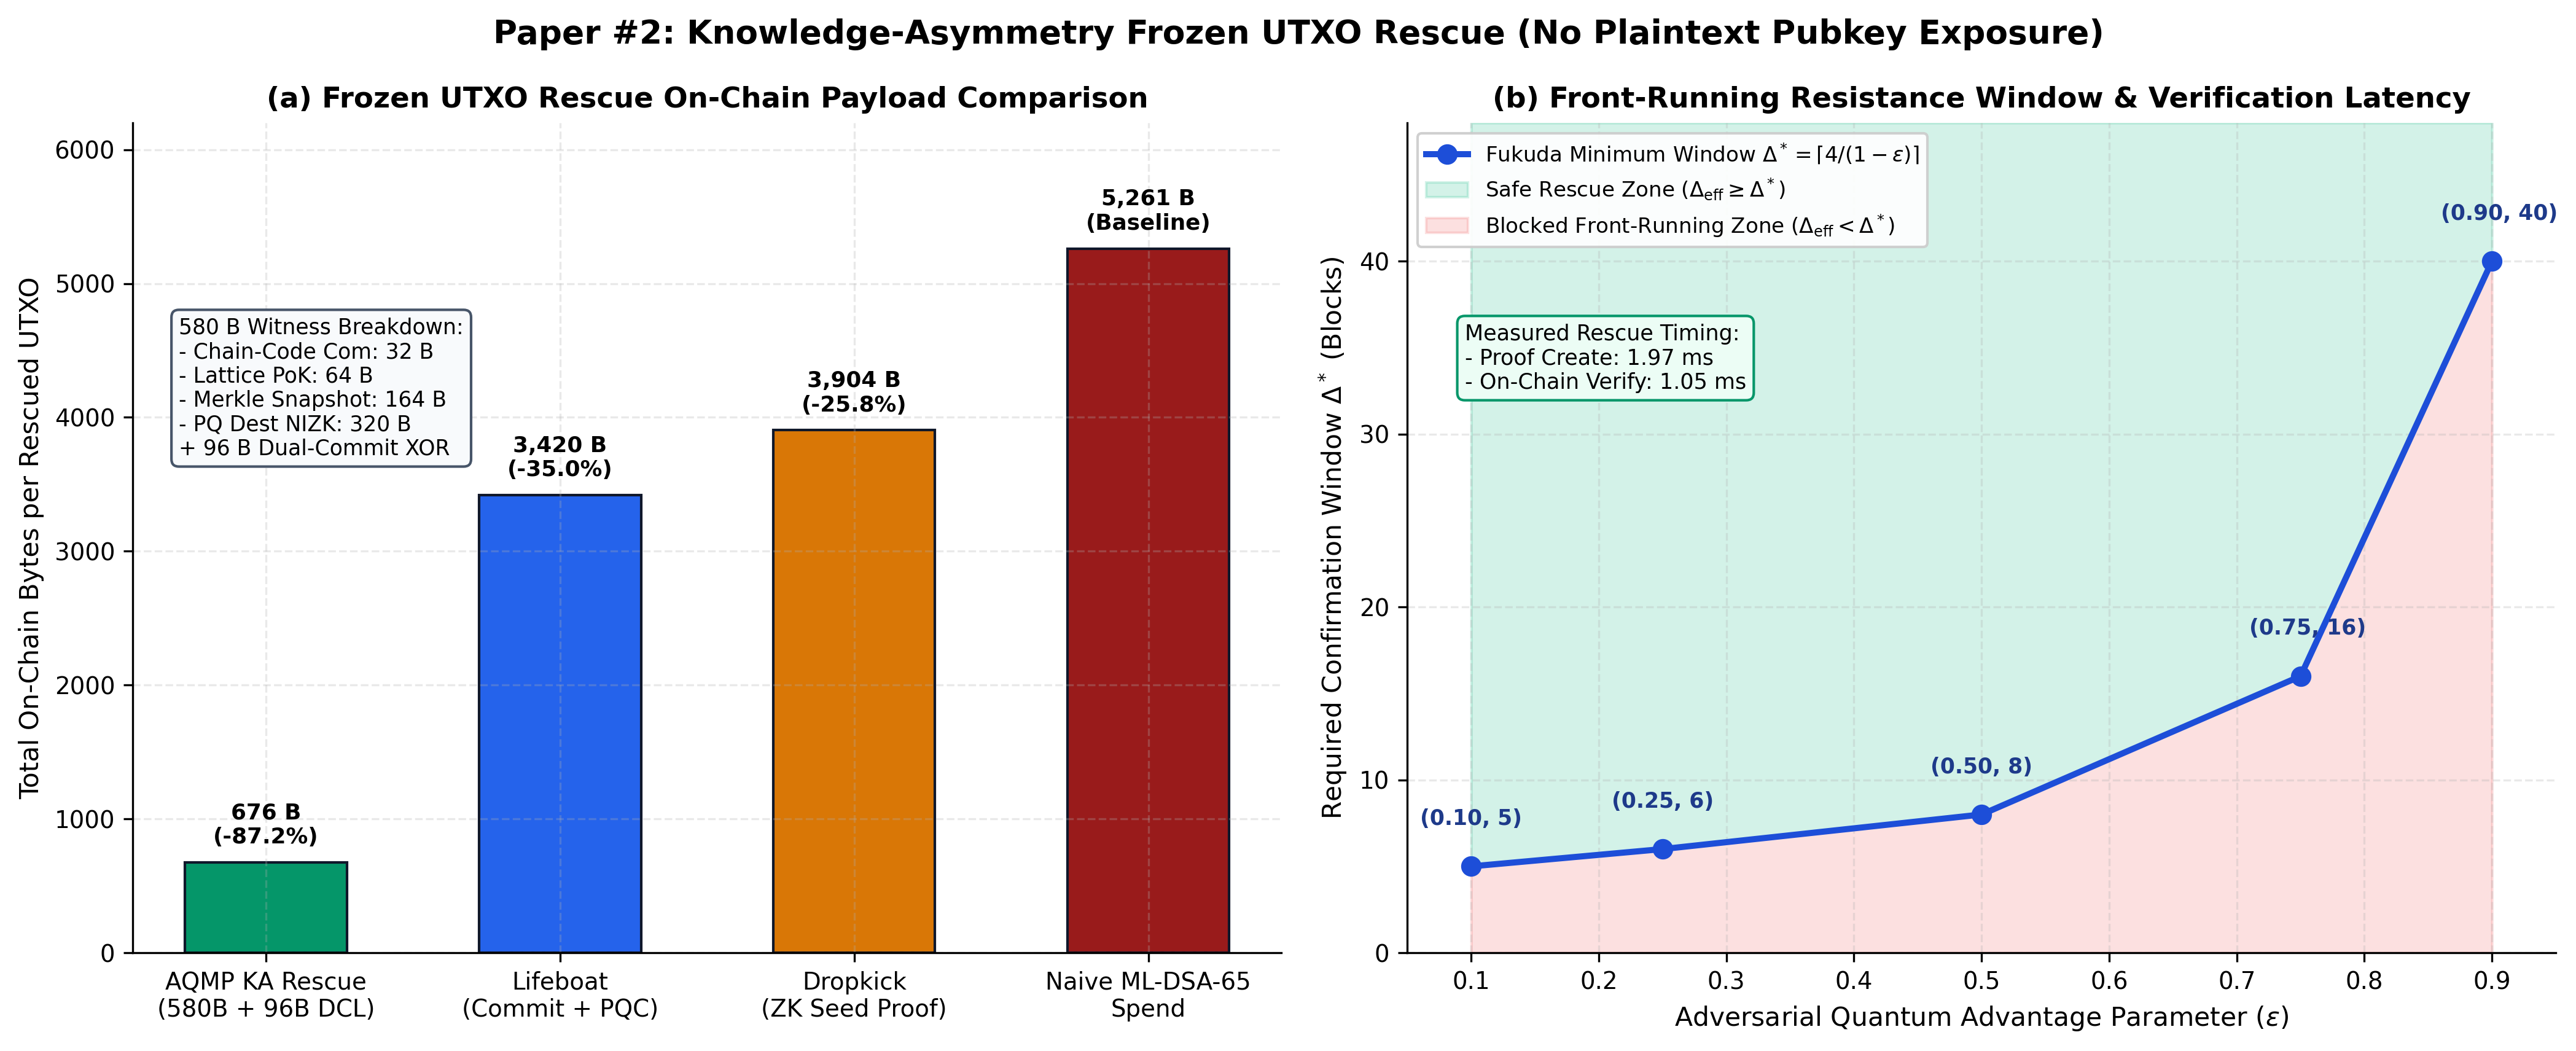
\includegraphics[width=0.95\textwidth]{figures/fig5_utxo_rescue_comparison.png}
\caption{Knowledge-Asymmetry frozen UTXO rescue byte footprint breakdown vs.\ Lifeboat, Dropkick, and Naive ML-DSA-65 (left) and Fukuda confirmation deadline boundary $\Delta^* = \lceil 4/(1-\epsilon)\rceil$ (right).}
\label{fig:rescue}
\end{figure*}

\section{Conclusion}
\label{sec:conclusion}

Stateless synthetic-PRF lattice threshold signing eliminates backup-restore nonce reuse for multi-zone custodians and compresses $3$-of-$5$ blocks to $11{,}300\text{ B}$ at $N = 250$. Pairing unhardened BIP-32 chain-code proofs with a $580\text{ B}$ lattice witness and a $96\text{ B}$ Dual-Commit XOR cycle rescues frozen UTXOs in $676\text{ B}$ without exposing elliptic-curve public keys or risking mempool destination hijacking.

\begin{thebibliography}{9}
\bibitem{aqmp2026} L. Kusuma, ``Breaking the Post-Quantum Cryptography Blockchain Migration Trilemma: AQMP v2.0,'' Zenodo Record 24303569, 2026.
\bibitem{bellare2006} M. Bellare and G. Neven, ``Multi-signatures in the plain public-key model and a general forking lemma,'' in \emph{ACM CCS}, 2006, pp. 390-399.
\bibitem{zhandry2019} M. Zhandry, ``How to record quantum queries, and applications to quantum indifferentiability,'' in \emph{CRYPTO}, 2019, pp. 239-268.
\bibitem{bip360} H. E. Hunter et al., ``BIP-360: Pay-to-Merkle-Root (P2MR),'' Bitcoin Improvement Proposals, 2025.
\bibitem{bip361} A. L. Corbit et al., ``BIP-361: Post-Quantum Migration and Legacy Output Sunsetting,'' Bitcoin Improvement Proposals, 2026.
\bibitem{nist2024} NIST, ``Module-Lattice-Based Digital Signature Standard (FIPS 204),'' 2024.
\end{thebibliography}

\end{document}
